% !TEX program = pdflatex
% !TEX root = main.tex

%----------------------------------------------------------------------------------------
\documentclass[a4paper,10pt]{article}

% Basic packages
\usepackage[utf8]{inputenc}
\usepackage{graphicx}
\usepackage{float}
\usepackage{amsmath}
\usepackage{amssymb}
\usepackage{amsthm}
\usepackage{multicol}
\usepackage{enumitem}
\usepackage{subcaption}
\usepackage{listings}
\usepackage{xcolor}
\usepackage{tikz}
\usetikzlibrary{positioning}
\usepackage[export]{adjustbox}
\usepackage[margin=2.5cm]{geometry}
\graphicspath{{images/}}
\usepackage{multirow}

% Load custom thesis style from config directory
\usepackage{config/thesis}

% Thesis information
\thesistype{Specialisation Project (VT1)}
\thesistitle{Platform for Investment Analysis}
\thesiscontext{Linear Programming Optimization Model for Integrated Energy Systems in Python}
\thesisdate{\today}
\thesissemester{HS2024}
\keywords{linear programming, quantitative modeling, python, strategic planning, optimization, asset valuation, power-flow, platform}

% Author information
\author{Rui Vieira}
\authorinstitute{Institute of Product Development and Production Technologies (IPP)}
\degree{Master of Science in Engineering}
\studyprogram{Business Engineering, MSc in Engineering}
\studyprogramlink{https://www.msengineering.ch/profiles/engineering-and-it/business-engineering}

% Supervisor information
\supervisorA{Dr. Andrea Giovanni Beccuti}
\supervisorAmail{giovanni.beccuti@zhaw.ch}
\supervisorAweb{https://www.zhaw.ch/en/about-us/person/becc}
\supervisorAinstitute{IEFE Model Based Process Optimisation}
\supervisorAinfo{%
    \supnameA\\
    \supinstituteA\\
    Email: \href{mailto:\supmailA}{\supmailA}\\
}

%----------------------------------------------------------------------------------------
\begin{document}

% Front
\begin{titlepage}
\begin{center}

\textup{\small {\bf \ttype} \\ \tsemester}\\
\vspace{1.9in}

% Title
\fontsize{20}{24}\selectfont
{\huge \textbf{\ttitle}}\\
\normalsize \tcontext\\
\vspace{1.9in}

% Submitted by
\emph{Submitted by} \\
\textbf{\authorname}\\
\authorinstitute\\
\vspace{.2in}

% Supervisor
\emph{Supervisor} \\
\textbf{\supnameA}\\
\supinstituteA
\vspace{1.9in}

% Study program
\emph{Study Program} \\
\textbf{\studyprog}\\
\vspace{0.2in}

% School logo

\includegraphics[width=0.2 \textwidth]{images/zhaw.png}\\
\vspace{.2in}

% Date
\tdate

\end{center}
\end{titlepage}
% !TEX root = ../main.tex

%----------------------------------------------------------------------------------------
% IMPRINT
%----------------------------------------------------------------------------------------

\thispagestyle{empty}
\vspace*{\fill}

\noindent
{\bfseries  \Large Imprint}
\vspace{0.75cm}

\begin{footnotesize}

% Project information
\begin{flushleft} 
\begin{tabular}{ @{}lp{0.64\textwidth}@{} } 
    \emph{Project:}  & \ttype\\ 
    \emph{Title}:    & \ttitle\\
    \emph{Author}:   & \authorname\\
    \emph{Date}:     & \tdate\\
    \emph{Keywords}: & \keywordnames\\
\end{tabular}
\end{flushleft}

\vspace{0.75cm}

% University information
\noindent
\begin{minipage}[t]{0.95\textwidth}
\begin{flushleft} 
\emph{Study program:}\\
\href{\studyproglink}{\studyprog}\\
\href{\univlink}{\univname}
\end{flushleft}
\end{minipage}

\vspace{1.1cm}

\noindent
\begin{minipage}[t]{0.50\textwidth}
\begin{flushleft} 
\emph{Supervisor:}\\
\supinfoA
\end{flushleft}
\end{minipage}
\begin{minipage}[t]{0.45\textwidth}

    \begin{flushleft} 
\ifdefempty{\supnameB}
{}
{
    \emph{Supervisor 2:}\\
    \supinfoB
}
\end{flushleft}
\end{minipage}


\end{footnotesize}

\newpage
% !TEX root = ../main.tex

%----------------------------------------------------------------------------------------
% ABSTRACT PAGE
%----------------------------------------------------------------------------------------



\begin{abstract}
This project presents a platform for investment analysis in energy systems, focusing on the optimization of asset management through linear programming techniques. The framework integrates DC Optimal Power Flow (DC-OPF) for network analysis with economic evaluation methods to support investment decisions in energy infrastructure.

The platform, implemented in Python, combines power system modeling with financial analysis tools to evaluate different investment scenarios. It features automated scenario generation, optimization of operational costs, and AI-assisted analysis of results. The methodology incorporates both technical constraints from power system operations and financial metrics such as Net Present Value (NPV) to provide comprehensive decision support.

Key features include modular architecture for extensibility, integration with industry-standard optimization solvers, and a flexible scenario analysis framework. The platform demonstrates practical applicability through case studies in energy infrastructure investment, showing how it can be used to evaluate complex investment decisions while considering both technical and economic factors.

\textbf{Keywords:} \keywordnames
\end{abstract}
\newpage

% Table of contents
\setcounter{tocdepth}{2}
\tableofcontents
\newpage

% Main content
\newpage
\section{Introduction}


% Context and motivation
% Problem statement
% Project objectives
% Brief overview of existing solutions/literature review
% Brief introduction to energy investment optimization and the need for automated analysis tools.

\subsection{Project Context}

\subsection{Objectives}
\begin{itemize}
    \item Develop a Python-based platform for energy investment analysis
    \item Implement linear programming optimization for asset management
    \item Investment analysis 
\end{itemize}
\newpage 

\newpage
\section{Theoretical Background}
\label{sec:theoretical_background}

\subsection{Linear Programming in Energy Systems}

At its core, our problem focuses on meeting electricity demand through optimal generation dispatch:
determining how much power each generator should produce to satisfy consumer demand while minimizing costs 
and respecting system constraints. This fundamental power systems challenge can be effectively modeled using 
Linear Programming (LP).
\begin{figure}[h]
    \centering
    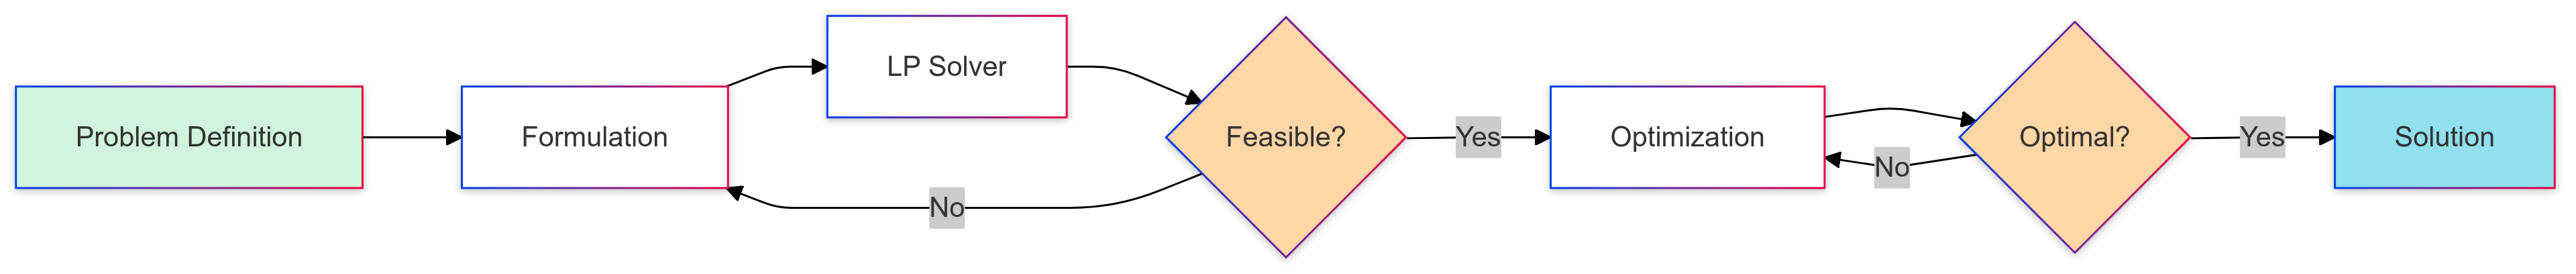
\includegraphics[width=0.8\textwidth]{images/lp_flowchart.png}
    \caption{LP optimization flowchart showing key steps from problem formulation to optimal solution.} \label{fig:lp_flowchart}
\end{figure}

Linear Programming enables modeling of key power system relationships - such as power balance 
(matching generation to demand), transmission limits, and generation constraints - as linear 
equations and inequalities. The basic structure of our optimization problem is:

\begin{itemize}
    \item \textbf{Objective}: Minimize total generation cost
    \item \textbf{Primary Decision}: How much power to generate at each plant
    \item \textbf{Key Constraint}: Total generation must meet demand at all times
    \item \textbf{System Constraints}: Respect network and equipment limitations
\end{itemize}

This can be expressed mathematically as:

\begin{equation}
    \min_{\mathbf{x}} \mathbf{c}^\top \mathbf{x} \quad \text{subject to} \quad A\mathbf{x} \leq \mathbf{b}
\end{equation}

\subsection{DC Optimal Power Flow}
The DC Optimal Power Flow (DC-OPF) extends the basic generation dispatch problem by incorporating network constraints.
It answers the question: "How should we distribute power generation across the network to meet demand
at minimum cost while respecting transmission line limits?" The DC-OPF achieves this by:
\begin{itemize}
    \item Modeling power flow through transmission lines
    \item Ensuring power balance at each network node
    \item Respecting both generation and transmission limits
\end{itemize}

The "DC" prefix indicates a linearized approximation of the full AC power flow equations, making the problem
 solvable using LP techniques~\cite{wood2013power}. This approximation is particularly effective for 
 high-voltage transmission planning~\cite{andersson2004power}.

\subsubsection{Key Assumptions}
The DC approximation makes four key simplifications:
\begin{itemize}
    \item Voltage magnitudes are fixed at 1.0 per unit
    \item Line resistances are negligible ($R \ll X$)
    \item Voltage angle differences are small
    \item Reactive power (power that oscillates between source and load without doing useful work) is ignored
\end{itemize}

These assumptions yield a simple relationship between power flow ($P_{ij}$) and voltage angles ($\theta$):
\begin{equation}
    P_{ij} = B_{ij}(\theta_i - \theta_j)
\end{equation}

\subsubsection{Mathematical Formulation}
The DC-OPF problem minimizes generation costs subject to network constraints. Each equation represents a 
physical aspect of power system operation:

\vspace{0.5cm}
\textbf{1. Power Balance} - The fundamental law of power systems
\begin{itemize}
    \item At each bus $i$, power in equals power out
    \item Generation minus demand equals net power flow to neighboring buses
    \item Determined by line susceptances and voltage angles
\end{itemize}
\begin{equation}
    \sum_{g \in \mathcal{G}_i} P_{g,t} - D_{i,t} = \sum_{j \in \mathcal{N}_i} B_{ij}(\theta_{i,t} - \theta_{j,t}) \quad \forall i \in \mathcal{N}, t \in \mathcal{T}
\end{equation}

\vspace{0.5cm}
\textbf{2. Cost Minimization} - Economic objective
\begin{itemize}
    \item Find optimal generation dispatch that minimizes total system cost
    \item Each generator has an associated marginal cost function (cost per unit of production)
\end{itemize}
\begin{equation}
    \min_{\mathbf{P_g}, \boldsymbol{\theta}} \sum_{g \in \mathcal{G}} \sum_{t \in \mathcal{T}} c_g P_{g,t}
\end{equation}

\vspace{0.5cm}
\textbf{3. Line Capacity} - Network limitations
\begin{itemize}
    \item Power flow must stay within thermal limits of transmission lines
    \item Bi-directional constraint (forward and reverse flow limits)
\end{itemize}
\begin{equation}
    -P_{ij}^{\max} \leq B_{ij}(\theta_{i,t} - \theta_{j,t}) \leq P_{ij}^{\max} \quad \forall (i,j) \in \mathcal{L}, t \in \mathcal{T}
\end{equation}

\vspace{0.5cm}
\textbf{4. Generator Limits} - Physical constraints
\begin{itemize}
    \item Each generator is limited by minimum and maximum output
    \item Generators may have time-varying limits
\end{itemize}
\begin{equation}
    P_{g}^{\min} \leq P_{g,t} \leq P_{g}^{\max} \quad \forall g \in \mathcal{G}, t \in \mathcal{T}
\end{equation}

\vspace{0.5cm}
\textbf{5. Reference Angle} - System reference
\begin{itemize}
    \item One bus sets the reference for voltage angles
    \item Typically chosen as the largest generator
\end{itemize}
\begin{equation}
    \theta_{\text{slack},t} = 0 \quad \forall t \in \mathcal{T}
\end{equation}

\subsubsection{Storage System Constraints}
The model includes battery storage systems with the following constraints:

\vspace{0.5cm}
\textbf{1. Energy Balance} - Storage state evolution
\begin{itemize}
    \item Tracks energy level over time
    \item Accounts for charging and discharging efficiencies
\end{itemize}
\begin{equation}
    E_{s,t+1} = E_{s,t} + \eta_c P_{c,s,t} - \frac{P_{d,s,t}}{\eta_d} \quad \forall s \in \mathcal{S}, t \in \mathcal{T}
\end{equation}

\vspace{0.5cm}
\textbf{2. Power Limits} - Operational boundaries
\begin{itemize}
    \item Maximum charging and discharging rates
    \item Cannot charge and discharge simultaneously
\end{itemize}
\begin{equation}
    0 \leq P_{c,s,t} \leq P_{c,s}^{\max} \quad \forall s \in \mathcal{S}, t \in \mathcal{T}
\end{equation}
\begin{equation}
    0 \leq P_{d,s,t} \leq P_{d,s}^{\max} \quad \forall s \in \mathcal{S}, t \in \mathcal{T}
\end{equation}

\vspace{0.5cm}
\textbf{3. Energy Capacity} - Storage limits
\begin{itemize}
    \item Maximum and minimum state of charge
    \item Often includes end-state condition
\end{itemize}
\begin{equation}
    E_{s}^{\min} \leq E_{s,t} \leq E_{s}^{\max} \quad \forall s \in \mathcal{S}, t \in \mathcal{T}
\end{equation}
\begin{equation}
    E_{s,T} = E_{s,0} \quad \forall s \in \mathcal{S}
\end{equation}

Where:
\begin{itemize}
    \item $E_{s,t}$: Energy stored in battery $s$ at time $t$
    \item $P_{c,s,t}, P_{d,s,t}$: Charging and discharging power
    \item $\eta_c, \eta_d$: Charging and discharging efficiencies
\end{itemize}

\newpage
\section{Methodology and Implementation}
% 4.1 System Architecture
    % Overall platform design
    % Component interaction
    % Data flow diagram
% 4.2 Core Components
    % Scenario definition system
    % DCOPF solver implementation
    % Investment calculations
    % AI integration for analysis
% 4.3 Technical Implementation
    % Used technologies and libraries
    % Code structure and organization
    % Key algorithms and their implementation

\subsection{System Architecture}
Description of the linear programming implementation.

\subsection{Core Components}
How different scenarios are generated and compared.

\subsection{Technical Implementation}
Implementation of AI-powered analysis features. 
\section{Results and Validation}
\subsection{Test Cases}
Description of validation scenarios.

\subsection{Performance Analysis}
Computational efficiency and scalability.

\subsection{Case Studies}
Real-world applications and insights. 
\newpage
\section{Discussion}
% 7.1 Platform Capabilities
    % Strengths and unique features
    % Computational performance
    % Flexibility and extensibility
% 7.2 Limitations and Future Work
    % Current limitations
    % Potential improvements
    % Future development opportunities

\subsection{Platform Capabilities}
Current functionality and limitations.

\subsection{Future Improvements}
Potential enhancements and extensions. 
\newpage
\section{Conclusion}
% Project achievements
% Key learnings
% Potential applications



% Appendices
\appendix
\section{Technical Documentation}
\subsection{Installation Guide}
\subsection{User Manual}
\subsection{API Reference}

\section{Mathematical Formulations}
\subsection{Optimization Model}
\subsection{Economic Calculations} 

% References
\newpage
\addcontentsline{toc}{section}{References}
\bibliographystyle{plain}
\bibliography{sections/refs}

\end{document}
%----------------------------------------------------------------------------------------

% GUIDELINES
% technical explanation structure
    % start, high-level concepts before diving into details
    % pattern:
        % 1. Purpose/Goal
        % 2. Input requirements
        % 3. Process/Algorithm
        % 4. Output format
        % 5. Example usage
    % key technical areas to focus on:
        % Scenario definition system
        % DCOPF solver integration
        % Multi-scenario analysis process
        % AI integration for analysis
        % Report generation system

% Professor Interests ?
    % Mathematical rigor in DCOPF implementation
    % Scalability of the solution
    % Validation of results
    % Innovation in combining:
        % Power systems
        % Investment analysis
        % AI-powered insights
        % Real-world applicability
        % Code quality and structure

% Focus order
%     2 system architecture and data flow
%     1 DCOPF implementation
%     3 investment analysis layer
%     4 AI integration
%     5 complete workflow with examples

%----------------------------------------------------------------------------------------